\begin{figure}[!t]
\centering
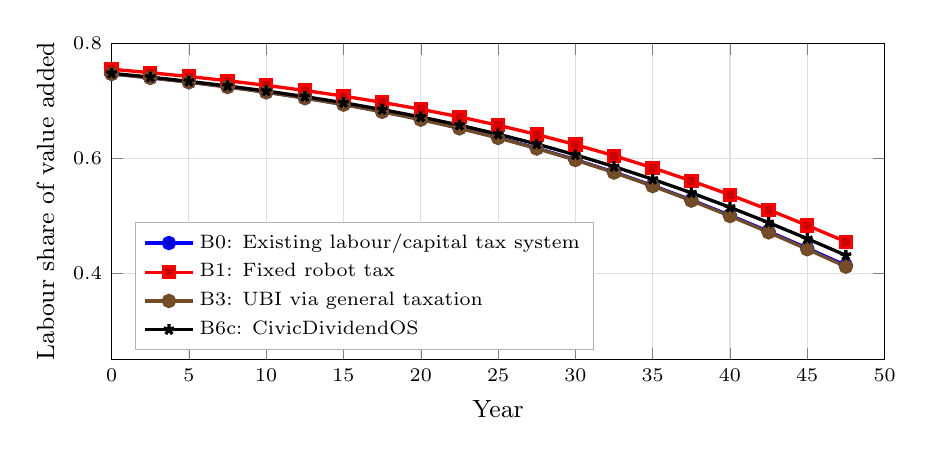
\begin{tikzpicture}
\begin{axis}[
  width=0.94\columnwidth, height=5.6cm,
  xlabel={Year}, ylabel={Labour share of value added},
  xmin=0, xmax=50, ymin=0.25, ymax=0.80,
  grid=major, grid style={black!12},
  legend pos=south west, legend cell align=left,
  legend style={font=\scriptsize, draw=black!30},
  label style={font=\small}, tick label style={font=\scriptsize},
  every axis plot/.append style={very thick, mark=none}
]
\addplot coordinates {(0.00,0.7467) (2.50,0.7399) (5.00,0.7323) (7.50,0.7240) (10.00,0.7149) (12.50,0.7047) (15.00,0.6935) (17.50,0.6811) (20.00,0.6675) (22.50,0.6524) (25.00,0.6358) (27.50,0.6175) (30.00,0.5976) (32.50,0.5759) (35.00,0.5525) (37.50,0.5274) (40.00,0.5008) (42.50,0.4727) (45.00,0.4436) (47.50,0.4136)};
\addlegendentry{B0: Existing labour/capital tax system}
\addplot coordinates {(0.00,0.7547) (2.50,0.7486) (5.00,0.7420) (7.50,0.7347) (10.00,0.7266) (12.50,0.7177) (15.00,0.7079) (17.50,0.6971) (20.00,0.6851) (22.50,0.6719) (25.00,0.6573) (27.50,0.6412) (30.00,0.6236) (32.50,0.6043) (35.00,0.5833) (37.50,0.5606) (40.00,0.5363) (42.50,0.5104) (45.00,0.4831) (47.50,0.4547)};
\addlegendentry{B1: Fixed robot tax}
\addplot coordinates {(0.00,0.7465) (2.50,0.7397) (5.00,0.7321) (7.50,0.7238) (10.00,0.7146) (12.50,0.7044) (15.00,0.6932) (17.50,0.6807) (20.00,0.6670) (22.50,0.6519) (25.00,0.6352) (27.50,0.6168) (30.00,0.5968) (32.50,0.5750) (35.00,0.5515) (37.50,0.5262) (40.00,0.4994) (42.50,0.4711) (45.00,0.4417) (47.50,0.4114)};
\addlegendentry{B3: UBI via general taxation}
\addplot coordinates {(0.00,0.7475) (2.50,0.7409) (5.00,0.7336) (7.50,0.7256) (10.00,0.7168) (12.50,0.7071) (15.00,0.6964) (17.50,0.6846) (20.00,0.6717) (22.50,0.6575) (25.00,0.6418) (27.50,0.6246) (30.00,0.6058) (32.50,0.5854) (35.00,0.5634) (37.50,0.5398) (40.00,0.5146) (42.50,0.4880) (45.00,0.4601) (47.50,0.4311)};
\addlegendentry{B6c: CivicDividendOS}
\end{axis}
\end{tikzpicture}
\caption{Labour share of value added over the 50-year horizon (seed 0). The machine price falls throughout, so the labour share declines in every arm. Arms that raise the effective cost of automation at the margin (B1, B6c) slow the decline; the UBI arm (B3) redistributes income but does not alter the factor allocation, so its path is indistinguishable from the baseline.}
\label{fig:results}
\end{figure}
